\documentclass{standalone}
\usepackage{tikz}
\usepackage{pxfonts}

\usetikzlibrary{shadows, calc}

\begin{document}

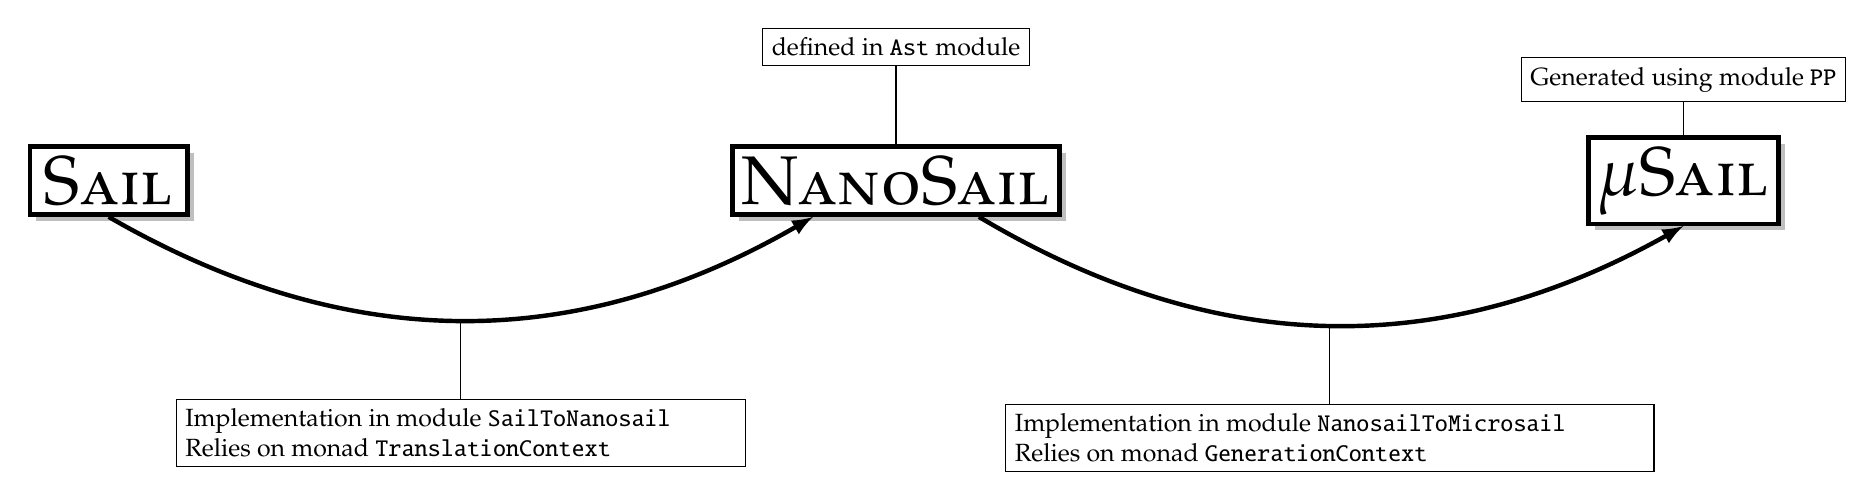
\begin{tikzpicture}[language/.style={minimum width=2cm,minimum height=8mm,draw,fill=white,drop shadow,font=\sc\Huge,ultra thick},
                    translation arrow/.style={-latex, ultra thick},
                    note/.style={draw,font=\small},
                   ]
  \node[language] (sail) at (0, 0) {Sail};
  \node[language] (nanosail) at (10, 0) {NanoSail};
  \node[language] (microsail) at (20, 0) {$\mu$Sail};

  \path[translation arrow] (sail.south) edge[bend right=30] node[midway,inner sep=0mm] (phase-1) {} ($ (nanosail.south west) ! 0.5 ! (nanosail.south) $);;
  \path[translation arrow] ($ (nanosail.south) ! 0.5 ! (nanosail.south east) $) edge[bend right=30] node[midway,inner sep=0mm] (phase-2) {} (microsail.south);

  \draw[thin] (phase-1) -- ++(0,-1) node[note,anchor=north] {
    \parbox{7cm}{
      Implementation in module \texttt{SailToNanosail} \\
      Relies on monad \texttt{TranslationContext}
    }
  };
  \draw[thin] (nanosail.north) -- ++(0,1) node[note,anchor=south] { defined in \texttt{Ast} module };
  \draw[thin] (phase-2) -- ++(0,-1) node[note,anchor=north] {
    \parbox{8cm}{
      Implementation in module \texttt{NanosailToMicrosail} \\
      Relies on monad \texttt{GenerationContext}
    }
  };
  \draw[thin] (microsail) -- ++(0,1) node[anchor=south,note] {
    Generated using module \texttt{PP}
  };
\end{tikzpicture}

\end{document}